\chapter{SPMonitor}

\todo{Add chapter introduction}

% This is the third result chapter which presents the first solution of the thesis.
% The solution is integrated into the overall concept introduced in Chapter 4 and
% it is technically based on the foundation described in Chapter 5.

% A thesis should provide at least two such solutions.

\todo{Explain purpose: maybe move motivation here; away from Analysis}

\subsection{Motivation}
The DrivingLicenseAuthorityKarlsruhe (DLAKa) wants to provide citizens with digital driving licenses,
which can, for example, be used to prove to a car rental company that they possess a valid driving license.
They hire the company ServiceProvider (SP) to develop and operate the system necessary for issuing and verifying
digital driving licenses. The contract specifies an initial payment for the development of the system
and afterward a yearly fee for the operation of the system.
After receiving the contract from DLAKa, SP starts designing the system
for DLAKa. Because SP has to operate the system on a fixed yearly budget,
they want to monitor the performance of the system to identify parts with excessive resource usage, which
incur additional costs. They identify the CPU and memory usage of the system as two technical metrics that should be monitored.
Additionally, DLAKa has asked them to provide the capability of monitoring business metrics for them.
DLAKa wants to know how many digital driving licenses are being issued and how often the issuance of a digital
driving license fails. To monitor both technical and business metrics, SP designs the ServiceProviderMonitor (SPMonitor) as a part
of the system for DLAKa which will provide all functionality for monitoring the specified metrics.

BestRental, a car rental company, has heard of DLAKa's plans for digital driving licenses
and wants to integrate them into its online rental system. Contrary to DLAKa, BestRental develops its
system in-house. Similarly to DLAKa, BestRental is interested in obtaining business metrics from its system.
They want to use these metrics to make business decisions like if they should increase the capacity of their fleet in the future.
For this purpose, BestRental designs an additional application called BestMonitor that will provide all the monitoring functionality.
In the beginning, they are only interested in one metric: How many active rentals are there?

For the design of SPMonitor, SP created two use cases: Present Metric and Collect Metric.
The relation of these use cases can be seen in the Use Case Diagram in Figure \ref{fig:use_case_monitoring_dlakaapp}.
Present Metric handles the use case of presenting the collected metrics to a user, this is described in Listing \ref{lis:use_case_description_present_metric}.
Collect Metric is concerned with how SPMonitor receives metrics for later presentation to a user, this is described in Listing \ref{lis:use_case_description_collect_metric}.

The metrics that will initially be monitored by SPMonitor are the number of issued digital driving licenses (NumDDL)
and the memory usage of the DLAKaApp (MemUse). The NumDDL metric is a business metric for DLAKa, while MemUse is
a technical metric that allows SP to monitor the performance of DLAKaApp.

\section{Analysis}

\todo{Introduction to Analysis}

\begin{figure}
	\centering
	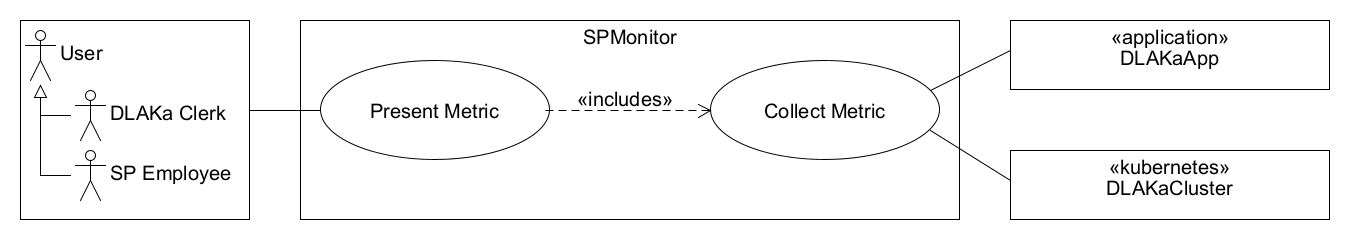
\includegraphics[width=\textwidth]{figures/2.1_use_case_spmonitor.png}
	\caption{Use Case Diagram: SPMonitor}
	\label{fig:use_case_monitoring_dlakaapp}
\end{figure}

\subsection{Use Case Present Metric}
\todo{Elaborate}

\begin{lstlisting}[caption = {Use Case Description: Present Metric}, label = {lis:use_case_description_present_metric}, style = kit-cm, language=]
Title: Present Metric

Primary Actors: DLAKa Clerk

Preconditions:
- SPMonitor has the NumDDL metric configured

Flow:
1. DLAKa Clerk opens the dashboard for the NumDDL metric
2. SPMonitor retrieves all stored values for the NumDDL metric
3. SPMonitor displays the values in a graph

Alternative Flows:
2a. SPMonitor has no values stored for the NumDDL metric
2a1. SPMonitor displays a message that the NumDDL metric has no stored values

Information Requirements:
- Values for the NumDDL metric
\end{lstlisting}

\subsection{Use Case Collect Metric}
\todo{Elaborate}

\begin{lstlisting}[caption = {Use Case Description: Collect Metric}, label = {lis:use_case_description_collect_metric}, style = kit-cm, language=]
Title: Collect Metric

Secondary Actors: DLAKaApp, DLAKaCluster

Preconditions:
- DLAKaApp is set up to collect the NumDDL metric
- DLAKaCluster is set up to collect the MemUse metric
- DLAKaApp is running inside of the DLAKaCluster
Postconditions:
- SPMonitor has values stored for NumDDL and MemUse

Flow:
1. SPMonitor sends a request to DLAKaApp for the NumDDL metric
2. DLAKaApp replies with a value for the NumDDL metric
3. SPMonitor receives the reply
4. SPMonitor stores the value for the NumDDL metric
5. SPMonitor sends a request to DLAKaCluster for the MemUse metric
6. DLAKaCluster replies with a value for the MemUse metric
7. SPMonitor receives the reply
8. SPMonitor stores the value for the MemUse metric

Alternative Flows:
2a. DLAKaApp replies with an error message
2a1. SPMonitor receives the error message
2a2. SPMonitor retries to request the NumDDL metric
6a. DLAKaCluster replies with an error message
6a1. SPMonitor receives the error message
6a2. SPMonitor retries to request the MemUse metric

Information Requirements:
- Value for the NumDDL metric
- Value for the MemUse metric
\end{lstlisting}

\todo{Summarize Analysis}

\section{Design}

\todo{Introduction for Design}

\subsection{Metrics Definition}

\subsection{Selecting the Tools}

As explained in Chapter \ref{cha:technical_foundation}, a monitoring system consists of three parts:
The Data Source, Data Sink and a tool for visualization.
The data source is the core of a monitoring system. It is responsible for collecting the monitoring data
and dictates the needs for the data sink as well as the possibilities for the visualization.
Because of its central role, the data source will be the first component of the monitoring system that will be chosen
and the rest of the monitoring system will be chosen to best fit with and support the data source.

In order for the chosen data source to best fit the needs of SPMonitor, it needs to fulfill some requirements
which stem from SPMonitor's use cases. The first requirement for the data source is that it should be built
to support the use cases of SPMonitor. Tools that are built for different purposes but could be used for SPMonitor's
use cases, will be less preferable than tools that are designed for SPMonitor's use cases.
Secondly, the data source should be free to use. This requirement mostly stems from the scope of this work
as a bachelor's thesis without any funding.
Additionally, the data source needs to be able to collect technical metrics as well as business metrics.
While technical metrics can be gathered from most cloud environments automatically, business metrics
require the instrumentation of the source code of the monitored services. Many data sources can in theory
instrument service but they often use additional tools like OpenTelemetry for this. Because SPMonitor aims
to be as slim as possible, to reduce complexity, data sources that can instrument services on their own without
the need for an additional tool, will be preferred over data sources that can not do that.
Lastly, the data source needs to support two different cloud environments: Kubernetes for the on-premise parts
of DLAKaApp and Microsoft Azure for the decentralized identity part of DLAKaApp.

These six requirements for the data source are listed in Table \ref{tab:data_source_requirements}.
Requirements R2 through R6 are hard requirements, meaning that a data source that does not fulfill them
will not be chosen. Requirement R1 is a soft requirement that is meant as an orientation and does directly
lead to the elimination of a data source.

\begin{table}[]
\centering
\begin{tabular}{c|l}
Key & Requirements \\
\hline
R1 & Purpose \\
R2 & Licensing \\
R3 & Technical metrics \\
R4 & Business metrics \\
R5 & Kubernetes \\
R6 & Microsoft Azure \\
\end{tabular}
\caption{}
\label{tab:data_source_requirements}
\end{table}

The data sources that will be compared according to the requirements in Table \ref{tab:data_source_requirements} stem
from the paper \enquote{A Survey on Observability of Distributed Edge {\&} Container-Based Microservices}
by Usman et al. \cite{ToolSurvey}. The list from that survey was supplemented with one additional entry,
the TICK (Telegraf, InfluxDB, Chronograf, Kapacitor) stack. Any entries that do not support metrics or are purely research projects were eliminated.
Lastly, the entry for Kibana was changed to ELK for the ELK (ElasticSearch, LogStash, Kibana) stack.
The complete overview of all analyzed tools can be seen in Table \ref{tab:data_source_comparison}.

\begin{table}[]
\begin{tabular}{l|c|c|c|c|c|c}
Name & R1 & R2 & R3 & R4 & R5 & R6 \\
\hline
Apache SkyWalking		 & Performance & Free & \cmark & \cmark & \cmark & \xmark \\
Cilium					 & Networking & Free & \cmark & \xmark & \cmark & \cmark \\
Datadog					 & SaaS & Paid & \cmark & \cmark & \cmark & \cmark \\
Dynatrace				 & PaaS & Paid & \cmark & \xmark & \cmark & \cmark \\
ELK						 & Searching & Paid & \cmark & \xmark & \cmark & \cmark \\
Honeycomb				 & Debugging & Paid & \cmark & \cmark & \cmark & \cmark \\
Instana					 & Incidence Management & Paid & \cmark & \xmark & \cmark & \cmark \\
Monasca					 & MaaS & Free & \cmark & \xmark & \cmark & \xmark \\
New Relic				 & PaaS & Paid & \cmark & \cmark & \cmark & \cmark \\
\rowcolor{lightgray}
OpenTelemetry			 & Monitoring & Free & \cmark & \cmark & \cmark & \cmark \\
\rowcolor{lightgray}
Prometheus				 & Monitoring & Free/Paid & \cmark & \cmark & \cmark & \cmark \\
Scalyr					 & PaaS & Paid & \cmark & \xmark & \cmark & \xmark \\
SolarWinds				 & PaaS & Paid & \cmark & \xmark & \cmark & \cmark \\
Splunk					 & Resilience & Paid & \cmark & \cmark & \cmark & \cmark \\
Sumo Logic				 & Analytics & Paid & \cmark & \cmark & \cmark & \cmark \\
\rowcolor{lightgray}
TICK					 & Time Series Data & Free/Paid & \cmark & \cmark & \cmark & \cmark \\
\end{tabular}
\caption{Comparison of data sources}
\label{tab:data_source_comparison}
\end{table}

The three final candidates for use in SPMonitor can be seen highlighted in Table \ref{tab:data_source_comparison}.
They are OpenTelemetry, Prometheus, and the TICK stack.
OpenTelemetry is a standalone solution for the collection of metrics. 
It provides many client libraries to instrument service for business metrics and can integrate
with most data sinks and visualization tools.
Prometheus is commonly used in combination with the LGTM (Loki Grafana Tempo Mimir) stack.
Loki is a service for handling logs, Tempo is responsible for handling traces, Grafana is used for visualization and Mimir provides
long-term storage for Prometheus. Prometheus itself is responsible for the collection of metrics.
As this work only considers metrics, the full setup would use Grafana for visualization, Prometheus as the data source, and Mimir
as the data sink. As Mimir only provides Prometheus with an interface to a storage system and is itself not one, it can be paired with MinIO
a free-to-use object storage system.
The TICK stack consists of four different tools: Telegraf, InfluxDB, Chronograf, and Kapacitor.
Telegraf is responsible for collecting metrics from the monitored services. The collected metrics are then forwarded
to InfluxDB, the storage component of the stack, and Kapacitor which is responsible for data processing.
Chronograf provides the interface to visualize and analyze the collected metrics.

From these three options, Prometheus together with Grafana, Mimir, and MinIO was chosen for SPMonitor.
Unlike OpenTelemetry, Prometheus provides easy integration with its data sink and visualization tool as
they were built to work together. OpenTelemetry on the other hand is a standalone solution meant to enhance
other tools which do not collect metrics themselves. The TICK stack provides the same integration benefit compared
to OpenTelemetry. The decision between Prometheus and the TICK stack is not as straightforward.
Both fulfill all requirements, offer extensibility options through plugins for different data sources
and pre-built visualizations, and they are both open-source projects which can be freely used.
One difference between them is that there exists a provider solution for managing Grafana with Crossplane.
This does not seem to exist for the TICK stack. Crossplane will be used to provision and operate the cloud
services of DLAKaApp and SPMonitor. Therefore Grafana and Prometheus are chosen for SPMonitor as they offer tools
for integrating them with Crossplane compared to the TICK stack. The final selection of tools can be seen in Figure \ref{fig:spmonitor_tech_stack}.

\begin{figure}
	\centering
	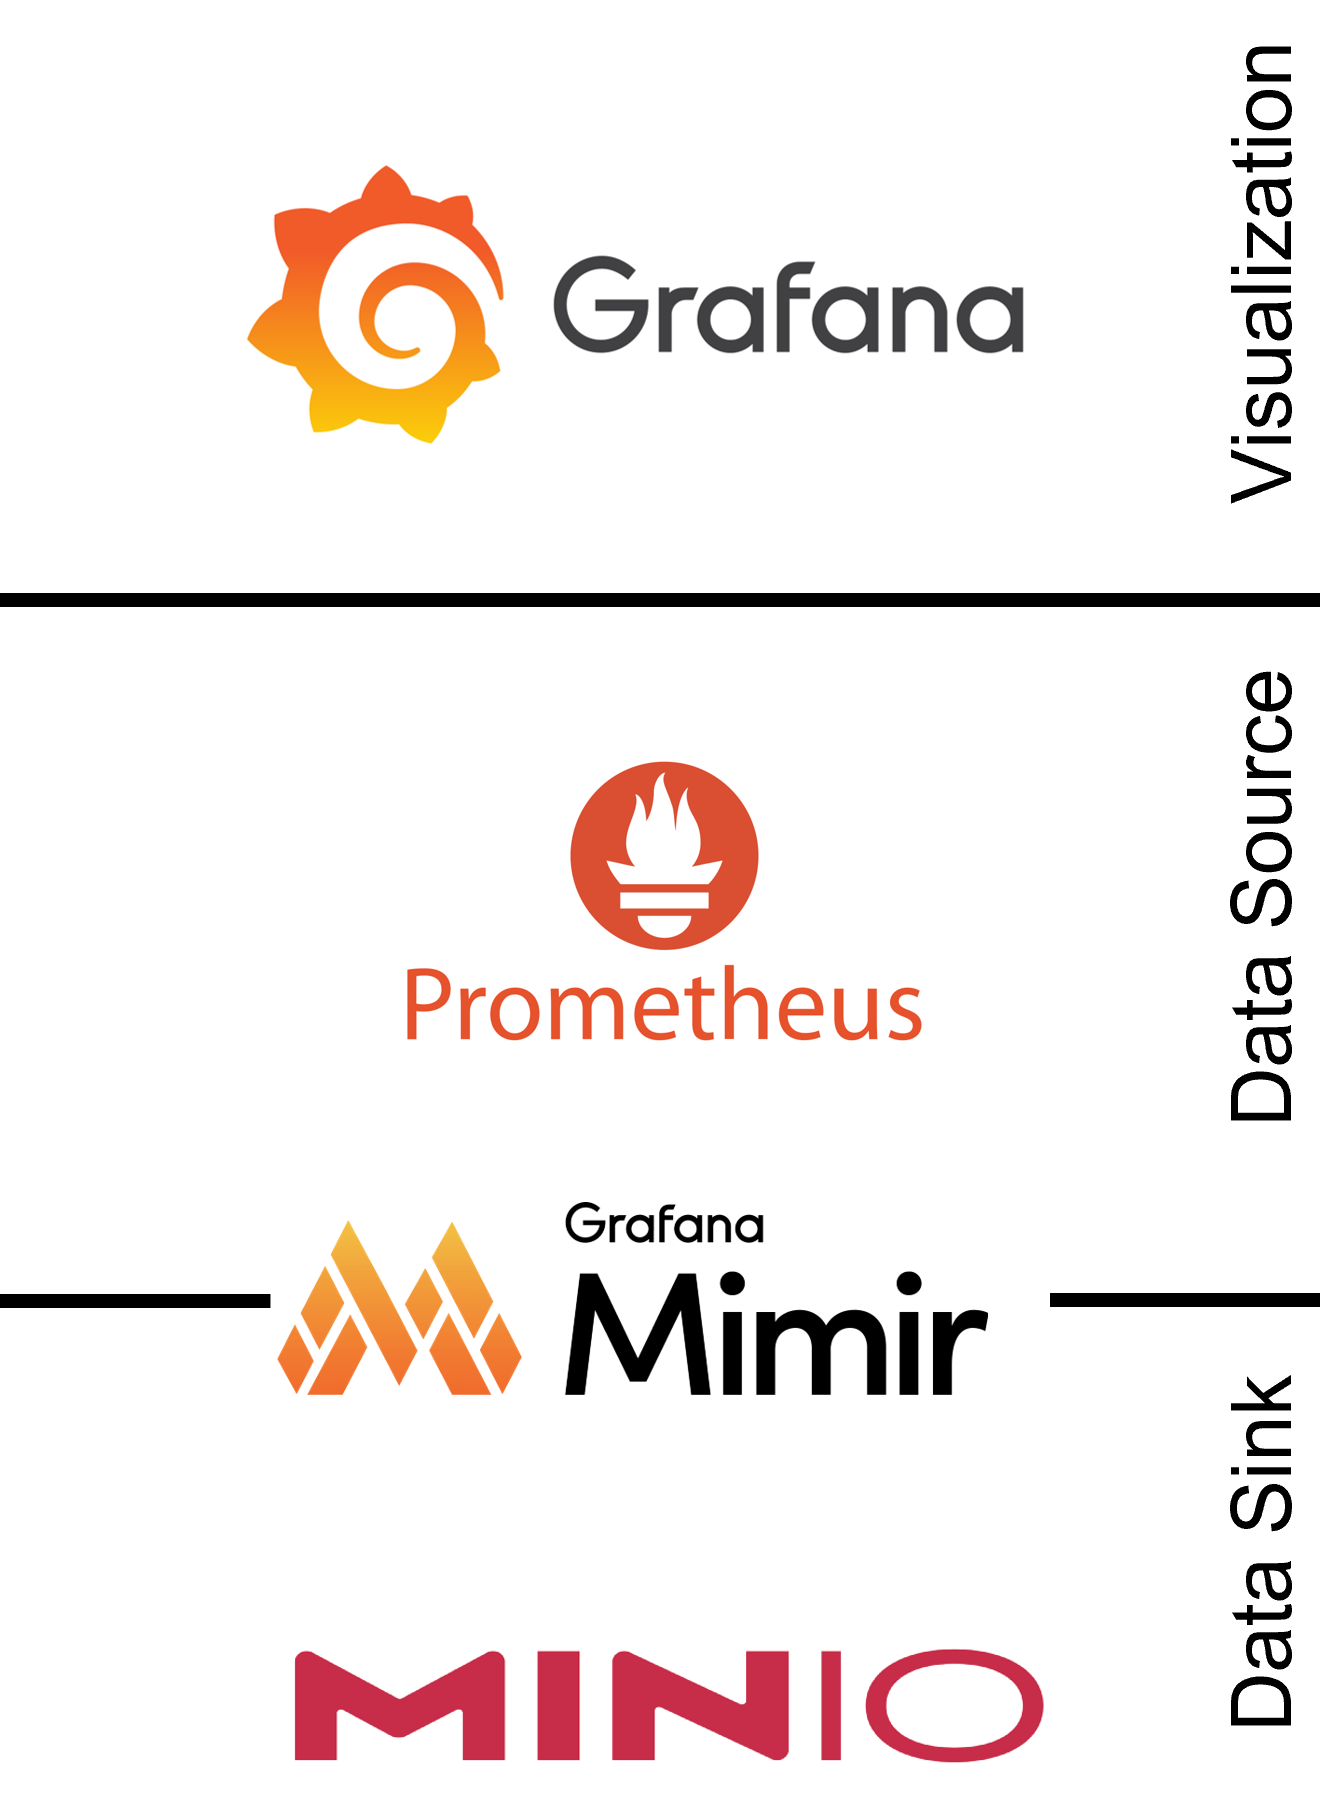
\includegraphics[width=0.4\textwidth]{figures/spmonitor_tech_stack.png}
	\caption{SPMonitor Technology Stack}
	\label{fig:spmonitor_tech_stack}
\end{figure}

\subsection{Architecture}

\todo{Explain SPS Architecture}

\subsection{API Specification}

\subsection{DevOps Concept}

\begin{figure}[h]
	\centering
	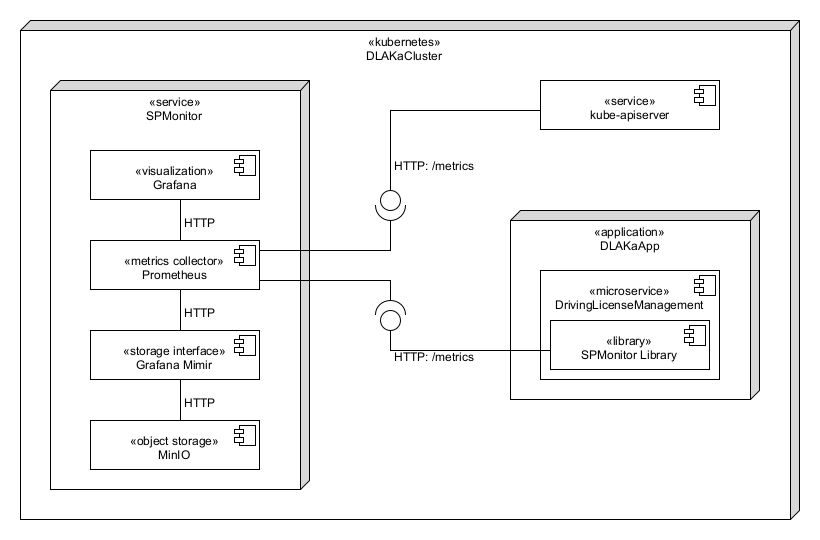
\includegraphics[width=\textwidth]{figures/sps_spmonitor.png}
	\caption{SystemPlusSoftware SPMonitor}
	\label{fig:sps_spmonitor}
\end{figure}

\section{Implementation}